\fancyhead{}
\fancyfoot{}


\lhead{Configurar VPN}
\subsection{Configuraci�n VPN Cliente}

Escoger el men� \textbf{New Terminal} $\rightarrow$ \textbf{system reset-configuration}\\
\begin{figure}[htb]
\begin{center}
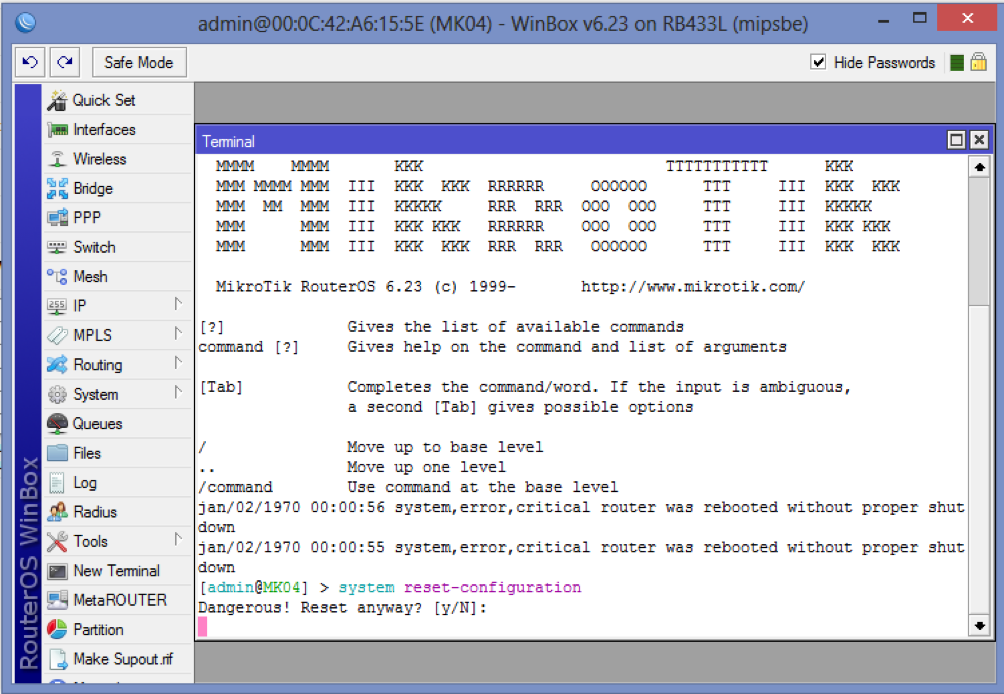
\includegraphics[scale = .5]{./figuras/figura092.png}
\caption{Remover configuraciones}
\label{remover-configuraciones}
\end{center}
\end{figure}
Escoger el men� \textbf{Remove Configuration} \\
\begin{figure}[htb]
\begin{center}
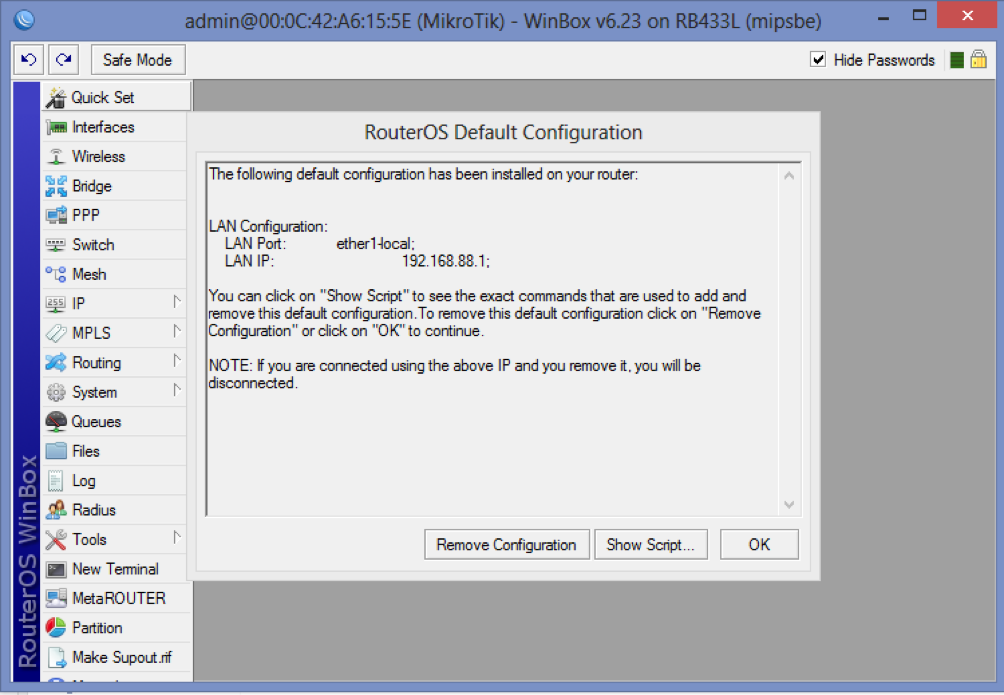
\includegraphics[scale = .5]{./figuras/figura093.png}
\caption{Remover configuraciones por defecto}
\label{remover-configuraciones-defecto}
\end{center}
\end{figure}

Escoger el men� \textbf{Wireless} $\rightarrow$  \textbf{wlan1} $\rightarrow$ \textbf{Wireless}\\
\begin{figure}[htb]
\begin{center}
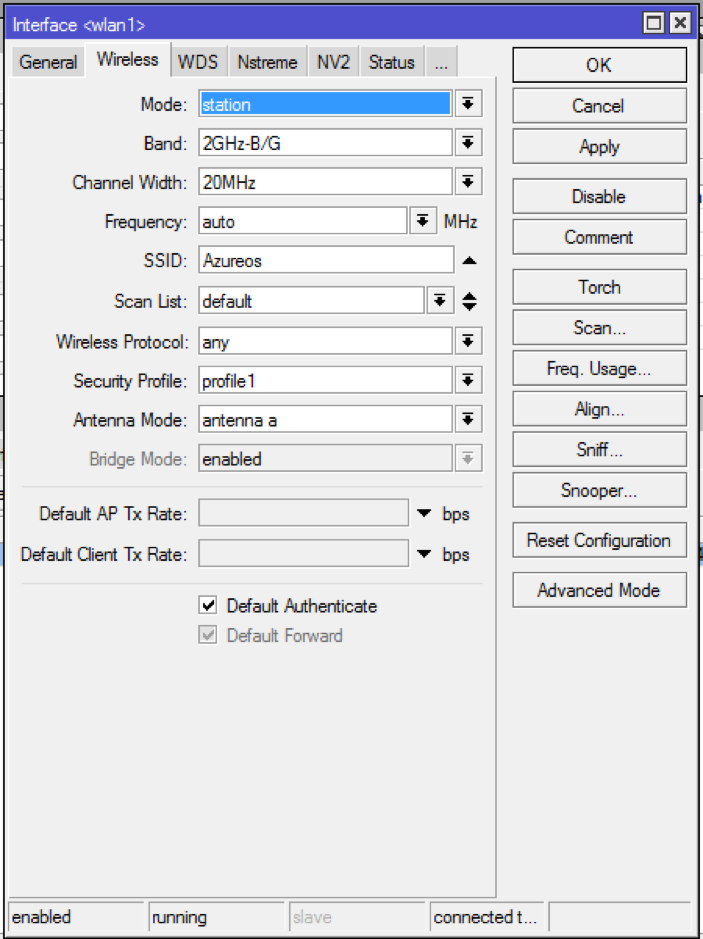
\includegraphics[scale = .5]{./figuras/figura094.png}
\caption{configurar WIFI}
\label{configurar-wifi}
\end{center}
\end{figure}

Escoger el men� \textbf{Wireless} $\rightarrow$  \textbf{Security Profiles}  $\rightarrow$ \textcolor{red}{\textbf{+}}\\

\begin{figure}[htb]
\begin{center}
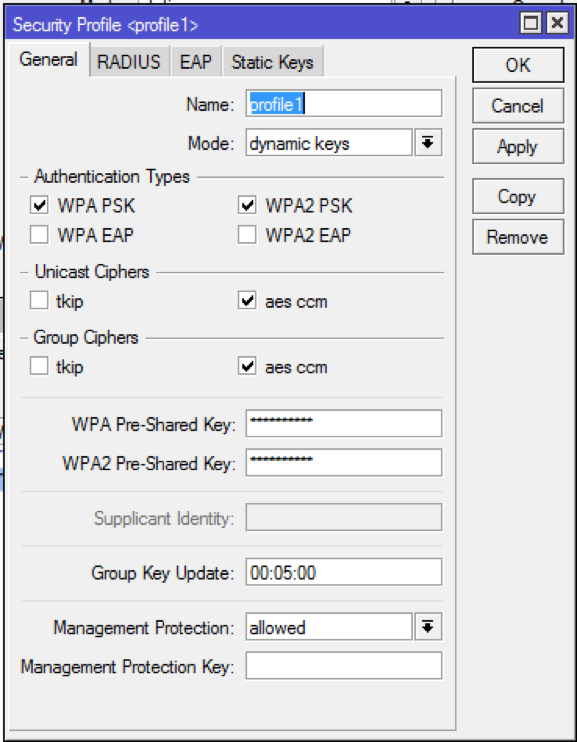
\includegraphics[scale = .5]{./figuras/figura095.png}
\caption{Perfil de seguridad del WIFI}
\label{perfil-seguridad-wifi}
\end{center}
\end{figure}

 Escoger el men� \textbf{IP} $\rightarrow$  \textbf{Address List}  
\begin{figure}[htb]
\begin{center}
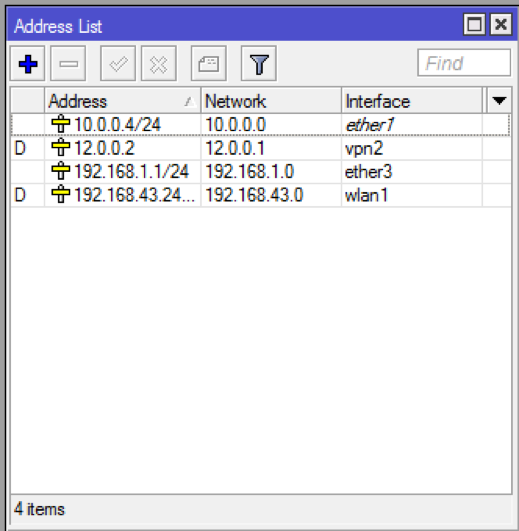
\includegraphics[scale = .5]{./figuras/figura096.png}

\caption{Lista de IP configurado MK4}
\label{lista-ip-configurado-mk4}
\end{center}
\end{figure}
 Escoger el men� \textbf{ppp} $\rightarrow$ \\
\begin{figure}[htb]
\begin{center}
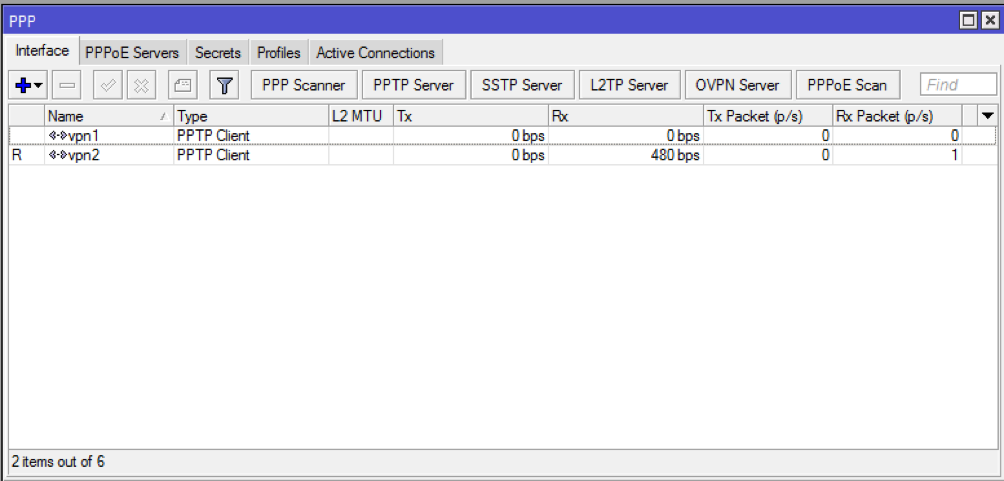
\includegraphics[scale = .5]{./figuras/figura097.png}
\caption{Lista de Discadores Clientes}
\label{lista-discadores-conectado}
\end{center}
\end{figure}